%%%%%%%%% O QUE É FECUNDIDADE MASCULINA %%%%%%%%%%


A fecundidade é um tema de grande relevância na demografia. Possui papel fundamental no estudo do ritmo do crescimento populacional, sendo uma das três componentes principais utilizadas no cálculo de projeções populacionais. É também a base de teorias demográficas que estudam padrões e mudanças na composição por grupos de idade da população e seus determinantes, como a transição demográfica \cite{FOZ2021metodos} e a transição da fecundidade \cite{mason1997explaining}.

No entanto, as formas de realizar a mensuração e análise da fecundidade são marcadas pela predominância da abordagem baseada apenas na fecundidade feminina, tanto nos indicadores produzidos a partir de inquéritos populacionais e registros administrativos no Brasil \cite{rede2002indicadores} e no mundo \cite{united2014principles, unies2004handbook}, como na literatura dos principais modelos e análises consolidados para abordagem no tema.Todavia, alguns autores \cite{zhang2010male, schoumaker2019male, joyner2012quality, paget1994relational, daumler2016men, dudel2019estimating} defendem a hipótese de que o estudo da fecundidade masculina é fundamental para a análise da transição demográfica e para o estudo da fecundidade humana de maneira completa.

Como afirma \citeonline{schoumaker2019male}, a falta de informações e de esforços na coleta de dados para a fecundidade masculina pode levar a uma falsa conclusão de que o comportamento reprodutivo de homens e mulheres é o mesmo. Pressupor, erroneamente, que assumem os mesmos níveis, padrões e mudanças ao longo do tempo, o que não se comprova, inclusive por estudos do próprio autor. Apesar disso, o campo na demografia que se debruça sobre a temática ainda é relativamente pouco explorado.

Analisando as razões pelas quais a demografia teria relegado a FM em prol da Fecundidade feminina, \citeonline{zhang2010male} identifica quatro categorias de argumentos tipicamente articulados na defesa de tal posicionamento, são eles: argumentos biológicos, metodológicos, sociológicos e teóricos. Em primeiro lugar, os argumentos biológicos giram em torno da ideia de que o ciclo reprodutivo feminino seria mais curto e bem definido (15-49) em comparação com o masculino (15-59\footnote{Não há um padrão bem definido, porém costuma ser adotado o intervalo de 15-59 anos, como na publicação do United Nations no Demographic Yearbook 2012. Fonte: https://unstats.un.org/unsd/demographic/products/dyb/dyb2012/notes/notes11.pdf}) e que, o espaçamento e o número de crianças teriam uma variação menor entre as mulheres, devido ao tempo de concepção feminino que impõe um intervalo mínimo de cerca de 1 a 2 anos para reprodução para as mulheres, enquanto para os homens não há esse limitador, levando a uma preferência por investigar a fecundidade através das mulheres. 

O fator metodológico (ou prático), como chama \citeonline{zhang2010male}, estaria associado ao padrão de coleta aplicado historicamente na demografia, no qual mulheres seriam mais fáceis de serem encontradas em casa em comparação aos seus companheiros. Complementarmente, é pressuposto que mulheres forneçam maior acurácia para variáveis associadas à fecundidade por estarem mais envolvidas nos eventos reprodutivos, o que faria delas fonte de informação mais confiável. Ainda entre as razões metodológicas para a FM ser deixada de lado pela maior parte do campo da demografia, \citeonline{zhang2010male} inclui a complexidade conceitual e técnica de inseri-la em modelos clássicos unissexuais (que consideram apenas um sexo, o feminino) como o modelo de população estável ou modelos para o estudo da fecundidade. Alguns autores têm se debruçado sobre essa questão \cite{li2022two,shyu2018mating,caswell2022formal}, mas ainda não existe um consenso sobre a melhor forma de como considerar a FM e fecundidade feminina em modelos demográficos.   


Sob o aspecto teórico, é escassa a produção na demografia que incluiu os homens nos estudos sobre os determinantes para a transição da fecundidade. Fatores como o casamento e o uso de contraceptivos costumam ser considerados apenas com foco nas mulheres. Pelo ponto de vista sociológico, enquanto mulheres são submetidas socialmente aos papéis ligados aos aspectos reprodutivos e às tarefas do cuidado, homens são socializados para não assumirem esse papel. Esse último aspecto, o sociológico, influencia os argumentos demográficos e metodológicos, uma vez que a demografia não é uma ciência desconectada do contexto social em que é produzida, sendo formada pela ótica, e muitas vezes pelos estereótipos, dos pesquisadores na produção de conhecimento, reproduzindo papéis de gênero socialmente difundidos \cite{watkins1993if}. Os aspectos metodológico e sociológico também se relacionam, visto que a escolha das mulheres como fonte confiável para os processos reprodutivos, inclusive para obtenção de informações relacionadas ao seu companheiro, está associado ao fato de elas estarem mais disponíveis em suas casas, consequência essa de terem as tarefas do cuidado incumbidas socialmente pelos papéis de gênero. Essas foram, segundo \citeonline{zhang2010male}, os principais argumentos associados a predominância da fecundidade feminina na demografia. 

Apesar das quatro razões elencadas por \citeonline{zhang2010male} para que a demografia, enquanto área, enfatizasse a fecundidade feminina, o estudo da fecundidade masculina não é algo recente. \apudonline{kuczynski1932fertility}{karmel1947relations}, em seu livro \textit{“Fertility and Reproduction. Methods of Measuring the Balance of Births and Deaths”} de 1932, já analisava os diferenciais reprodutivos de homens e mulheres. Nesse estudo encontrou diferentes taxas líquidas de fecundidade para homens e mulheres para a população francesa nos anos 1920-1923. 

Buscando analisar o desenvolvimento da literatura sobre o tema da FM, realizamos uma rápida busca na base indexadora \textit{“Coleção principal do Web of Science”(WoS)} pelas chaves de busca para os termos em inglês, em português e espanhol, delimitando com aspas: \textit{“male fertility”, “fecundidad masculina”} e “fecundidade masculina” e filtrando para a categoria \textit{WoS}: \textit{“demografia”}, encontramos o total de 36 resultados\footnote{No dia 15 de maio de 2024}.

\begin{grafico}
    \centering
    \caption{Publicação de documentos por ano, resultado da busca pela chave \textit{“male fertility”}, restringindo para área de pesquisa de “demografia”.}
    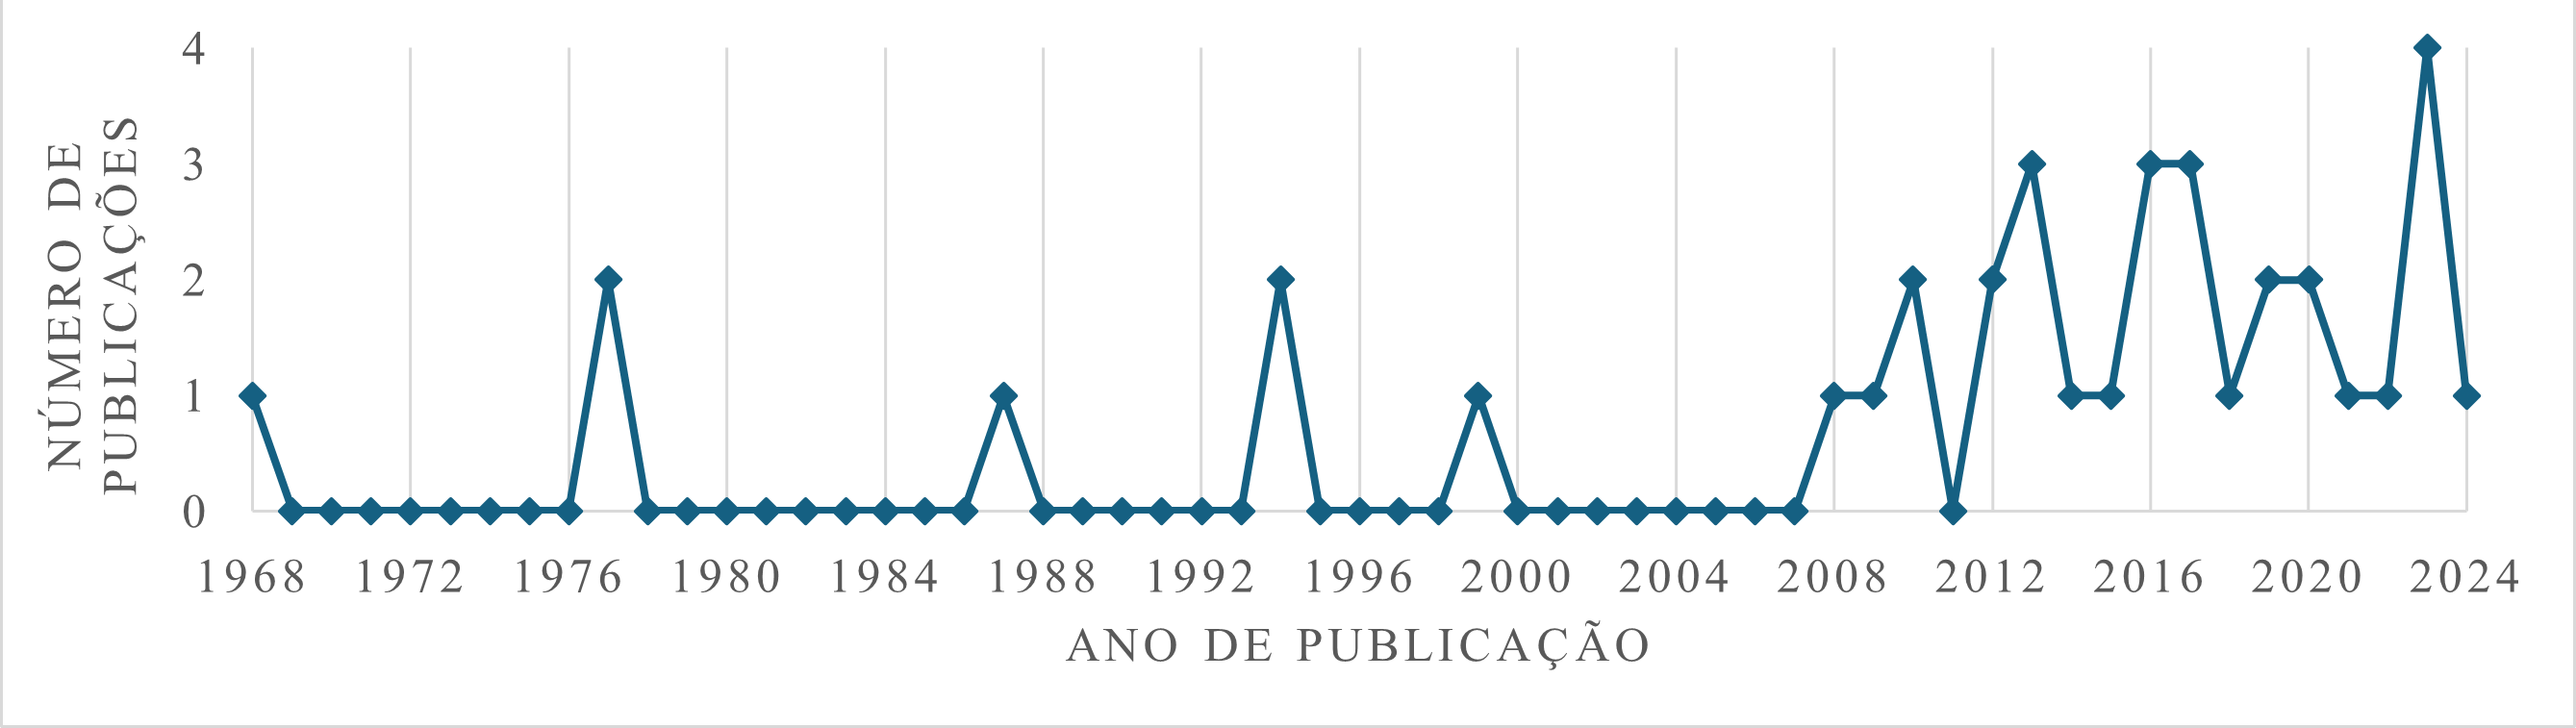
\includegraphics[scale=0.75]{imagens/grafico1.png}
    \fonte{Coleção principal do Web of Science, acesso em maio de 2024.}
    \label{graf:producao_anual}
\end{grafico}

O intervalo encontrado para a produção de artigos sobre FM na WoS foi de 1968 a 2024. Foram encontrados nesse indexador 36 documentos produzidos por 64 autores. A idade média dos textos foi de 13,5 anos, demonstrando que, apesar da frequência com que esses documentos são produzidos ter aumentado a partir de 2008, como é possível observar no Gráfico \ref{graf:producao_anual}, o campo teórico da FM já existe, pelo menos, desde 1968. Os países que mais concentraram publicações foram a Alemanha (11) e os Estados Unidos (10), seguidos pela Holanda (7), Inglaterra (4), México (2), França (1) e Índia (1), demonstrando que o estudo da temática continua concentrado em poucos países. Porém, foi possível observar que há um interesse crescente no estudo da FM.

